\begin{enumerate}
	\item задание.
	\begin{figure}[H]

		% Левый блок: таблицы истинности
		\noindent
		\begin{minipage}[t]{0.45\linewidth}
			\small Первая функция \\[0.5ex]
			\centering
			\begin{tabular}[t]{ccc|c}
				$x_1$ & $x_2$ & $x_3$ & $f_1$ \\
				\hline
				0 & 0 & 0 & 0 \\
				0 & 0 & 1 & 0 \\
				0 & 1 & 0 & 1 \\
				0 & 1 & 1 & 1 \\
				1 & 0 & 0 & 1 \\
				1 & 0 & 1 & 0 \\
				1 & 1 & 0 & 0 \\
				1 & 1 & 1 & 1 \\
			\end{tabular}

			\vspace{1.5em}

			\small Вторая функция \\[0.5ex]
			\centering
			\begin{tabular}[t]{cccc|c}
				$x_1$ & $x_2$ & $x_3$ & $x_4$ & $f_2$ \\
				\hline
				0 & 0 & 0 & 0 & 1 \\
				0 & 0 & 0 & 1 & 1 \\
				0 & 0 & 1 & 0 & 1 \\
				0 & 0 & 1 & 1 & 1 \\
				0 & 1 & 0 & 0 & 1 \\
				0 & 1 & 0 & 1 & 1 \\
				0 & 1 & 1 & 0 & 1 \\
				0 & 1 & 1 & 1 & 1 \\
				1 & 0 & 0 & 0 & 1 \\
				1 & 0 & 0 & 1 & 0 \\
				1 & 0 & 1 & 0 & 0 \\
				1 & 0 & 1 & 1 & 1 \\
				1 & 1 & 0 & 0 & 0 \\
				1 & 1 & 0 & 1 & 1 \\
				1 & 1 & 1 & 0 & 1 \\
				1 & 1 & 1 & 1 & 0 \\
			\end{tabular}
		\end{minipage}%
		\hfill % Пространство между блоками
		% Правый блок: диаграммы Вейча‑Карно
		\begin{minipage}[t]{0.48\linewidth}
			% Диаграмма для 3 переменных
			\small Диаграмма Вейча‑Карно ($f_1$) \\[0.5ex]
			\centering
\begin{tikzpicture}[karnaugh,disable bars,x=1\kmunitlength,y=1\kmunitlength,kmbar left sep=1\kmunitlength,grp/.style n args={4}{#1,fill=#1!30,minimum width= #2\kmunitlength,minimum height=#3\kmunitlength,rounded corners=0.2\kmunitlength,fill opacity=0.6,rectangle,draw}]
\karnaughmap{3}{$f$}{{$x_2$}{$x_1$}{$x_3$}}
{00101101}{
\draw[kmbox] (-0.5,2.5)
   node[below left]{$x_1$}
   node[above right]{$x_2$, $x_3$} +(-0.2,0.2)
   node[above left]{$f_1$};\draw (0,2) -- (-0.7,2.7);
\foreach \x/\1 in %
{0/00,1/01,2/11,3/10} {
   \node at (\x+0.5,2.2) {\1};
}
\foreach \y/\1 in %
{0/0,1/1} {
   \node at (-0.4,-0.5-\y+2) {\1};
}
   \node[grp={LogisimKMapColor0}{1.8}{0.8}](n0) at(3,1.5) {};
   \node[grp={LogisimKMapColor1}{0.8}{0.8}](n1) at(0.5,0.5) {};
   \node[grp={LogisimKMapColor2}{0.8}{1.8}](n2) at(2.5,1) {};
}
\end{tikzpicture}

			\vspace{8em}

			% Диаграмма для 4 переменных
			\small Диаграмма Вейча‑Карно ($f_2$) \\[0.5ex]
			\centering
\begin{tikzpicture}[karnaugh,disable bars,x=1\kmunitlength,y=1\kmunitlength,kmbar left sep=1\kmunitlength,grp/.style n args={4}{#1,fill=#1!30,minimum width= #2\kmunitlength,minimum height=#3\kmunitlength,rounded corners=0.2\kmunitlength,fill opacity=0.6,rectangle,draw}]
\karnaughmap{4}{$f$}{{$x_1$}{$x_3$}{$x_2$}{$x_4$}}
{1111111110010110}{
\draw[kmbox] (-0.5,4.5)
   node[below left]{$x_1$, $x_2$}
   node[above right]{$x_3$, $x_4$} +(-0.2,0.2)
   node[above left]{$f_2$};\draw (0,4) -- (-0.7,4.7);
\foreach \x/\1 in %
{0/00,1/01,2/11,3/10} {
   \node at (\x+0.5,4.2) {\1};
}
\foreach \y/\1 in %
{0/00,1/01,2/11,3/10} {
   \node at (-0.4,-0.5-\y+4) {\1};
}
   \node[grp={LogisimKMapColor0}{3.8}{1.8}](n0) at(2,3) {};
   \node[grp={LogisimKMapColor1}{0.8}{0.8}](n1) at(0.5,3.5) {};
   \node[grp={LogisimKMapColor1}{0.8}{0.8}](n2) at(0.5,0.5) {};
   \node[grp={LogisimKMapColor2}{0.8}{0.8}](n3) at(2.5,3.5) {};
   \node[grp={LogisimKMapColor2}{0.8}{0.8}](n4) at(2.5,0.5) {};
   \node[grp={LogisimKMapColor3}{0.8}{1.8}](n5) at(1.5,2) {};
   \node[grp={LogisimKMapColor4}{0.8}{1.8}](n6) at(3.5,2) {};
}
\end{tikzpicture}
		\end{minipage}

\end{figure}
\newpage

\begin{figure}[H]
	Минимизированные булевые функции:
\begin{itemize}
	\item[] $f_1 =  \overline{x_1}  \cdot x_2+x_1 \cdot  \overline{x_2}  \cdot  \overline{x_3} +x_2 \cdot x_3$ (О)
	\item[] $f_2 =  \overline{x_1} + \overline{x_2}  \cdot  \overline{x_3}  \cdot  \overline{x_4} + \overline{x_2}  \cdot x_3 \cdot x_4+x_2 \cdot  \overline{x_3}  \cdot x_4+x_2 \cdot x_3 \cdot  \overline{x_4} $ (О)
\end{itemize}
Перевод функции $f_1$ в базис Шеффера (Ш):
\begin{itemize}
	\item[] $x\ |\ y = \overline{x \cdot y},\ \ \ \overline{x}=x\ |\ x,\ \ \ x+y=\overline{x}\ |\ \overline{y},\ \ \ x \cdot y=\overline{x\ |\ y}$
\end{itemize}
\begin{enumerate}
	\item $f_1 =  \overline{\overline{x_2 \cdot (\overline{x_1} + x_3)+x_1 \cdot  \overline{x_2}  \cdot  \overline{x_3}}}$
	\item $f_1 =  \overline{(\overline{x_2 \cdot (\overline{x_1} + x_3)}) \cdot (\overline{x_1 \cdot  \overline{x_2}  \cdot  \overline{x_3}})}$
	\item $f_1 =  (x_2\ |\ \overline{\overline{(\overline{x_1}+x_3)}})\ |\ (x_1\ |\ (\overline{x_2} \cdot \overline{x_3}))$
	\item $f_1 =  (x_2\ |\ (\overline{x_1 \cdot \overline{x_3}}))\ |\ (x_1\ |\ (\overline{\overline{x_2}\ |\ \overline{x_3}}))$
	\item $f_1 =  (x_2\ |\ (x_1\ |\ (x_3\ |\ x_3)))\ |\ (x_1\ |\ (\overline{(x_2\ |\ x_2)\ |\ (x_3\ |\ x_3)}))$
	\item $f_1 =  (x_2\ |\ (x_1\ |\ (x_3\ |\ x_3)))\ |\ (x_1\ |\ (((x_2\ |\ x_2)\ |\ (x_3\ |\ x_3))\ |\ ((x_2\ |\ x_2)\ |\ (x_3\ |\ x_3))))$
\end{enumerate}
$f_1 =  (x_2\ |\ (x_1\ |\ (x_3|x_3)))\ |\ (x_1\ |\ (((x_2|x_2)\ |\ (x_3|x_3))\ |\ ((x_2|x_2)\ |\ (x_3|x_3))))$ (Ш)
\end{figure}
% \newpage
	\begin{figure}[H]
		\centering
		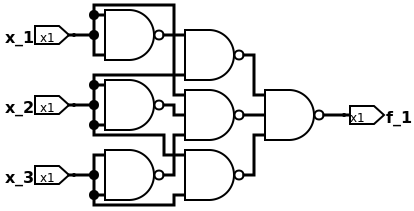
\includegraphics[width=17cm]{1.pdf}
		\caption{функция с счётчиком для проверки}
	\end{figure}

	\newpage
	\item задание.

	\begin{figure}[H]
		\centering
		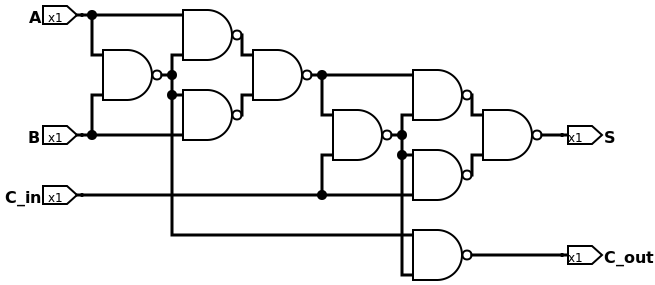
\includegraphics[width=17cm]{2-1.pdf}
		\caption{элемент summ}
	\end{figure}

	\begin{figure}[H]
		\centering
		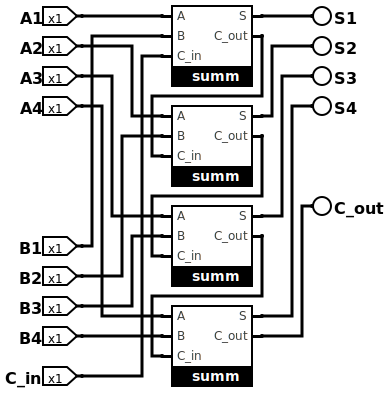
\includegraphics[width=17cm]{2-2.pdf}
		\caption{четырехразрядный полный сумматор}
	\end{figure}
	\newpage

	\item задание.
	\begin{figure}[H]
		\centering
		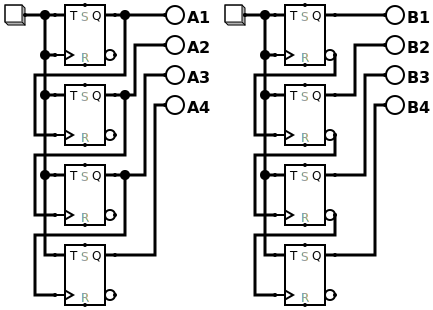
\includegraphics[width=17cm]{3.pdf}
		\caption{обратный счётчик слева и прямой справа}
	\end{figure}
	\newpage

	\item задание.
	\begin{figure}[H]
		\centering
		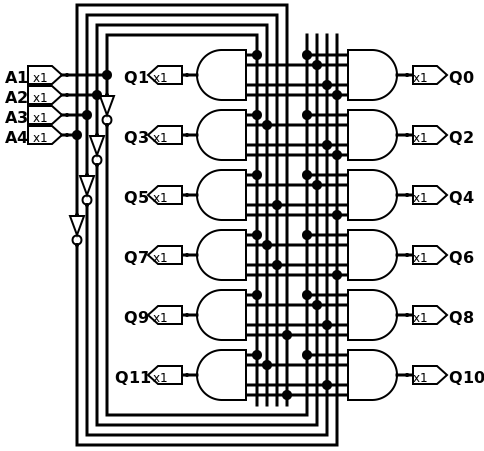
\includegraphics[width=17cm]{4-1.pdf}
		\caption{элемент dec}
	\end{figure}
	\newpage
	\begin{figure}[H]
		\centering
		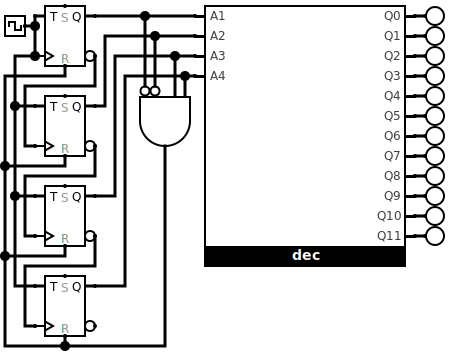
\includegraphics[width=17cm]{4-2.pdf}
		\caption{гирлянда}
	\end{figure}
	\newpage

\end{enumerate}
